\chapter{State of the Art}

\renewcommand{\chaptername}{Chapter}

\section*{Introduction}

The intralogistics sector is undergoing a significant transformation due to the 
integration of digital tools such as connected industries and robotics. The cluttered 
and highly dynamic nature of this environment makes it challenging to successfully 
implement robotic solutions.

The first steps in digitalizing logistic processes with robots involved the use of 
Automated Guided Vehicles (AGVs). First introduced in 1955, AGVs perform tasks like 
material handling. AGVs are managed by top-level software that handles task planning, 
providing the vehicles with intermediate waypoints to navigate from start to end points \cite{R7}. 

However, the decentralized decision-making approach of AGVs makes them 
unresponsive to changes in their environment. For example, AGVs localize themselves 
using specific and precise anchors physically located in their workspace. 

This localization mechanism helps them follow the assigned path. As a result, even 
a simple environmental change of the dispositionsrequires an update of the measurements 
and maps on  which the planning is based. Another example is that an AGV is unable to plan and 
execute a solution if it encounters an obstacle on its way to the goal or it arrives at a shifted 
destination. In such cases, 
the AGV’s reaction is to stop and wait for top-level instructions \cite{R8}. This behavior 
decreases productivity and disrupts the planned sequence of tasks until an intervention is managed.

To overcome these disadvantages of AGVs, Autonomous Mobile Robots (AMRs) were introduced. 
AMRs are equipped with a decentralized control system, enhanced perception of their 
surroundings through more complex hardware, and advanced software to manage and integrate 
these hardware additions (Figure \Ref{AMR-VS-AGV}).

\begin{figure}[H]
    \begin{center}
       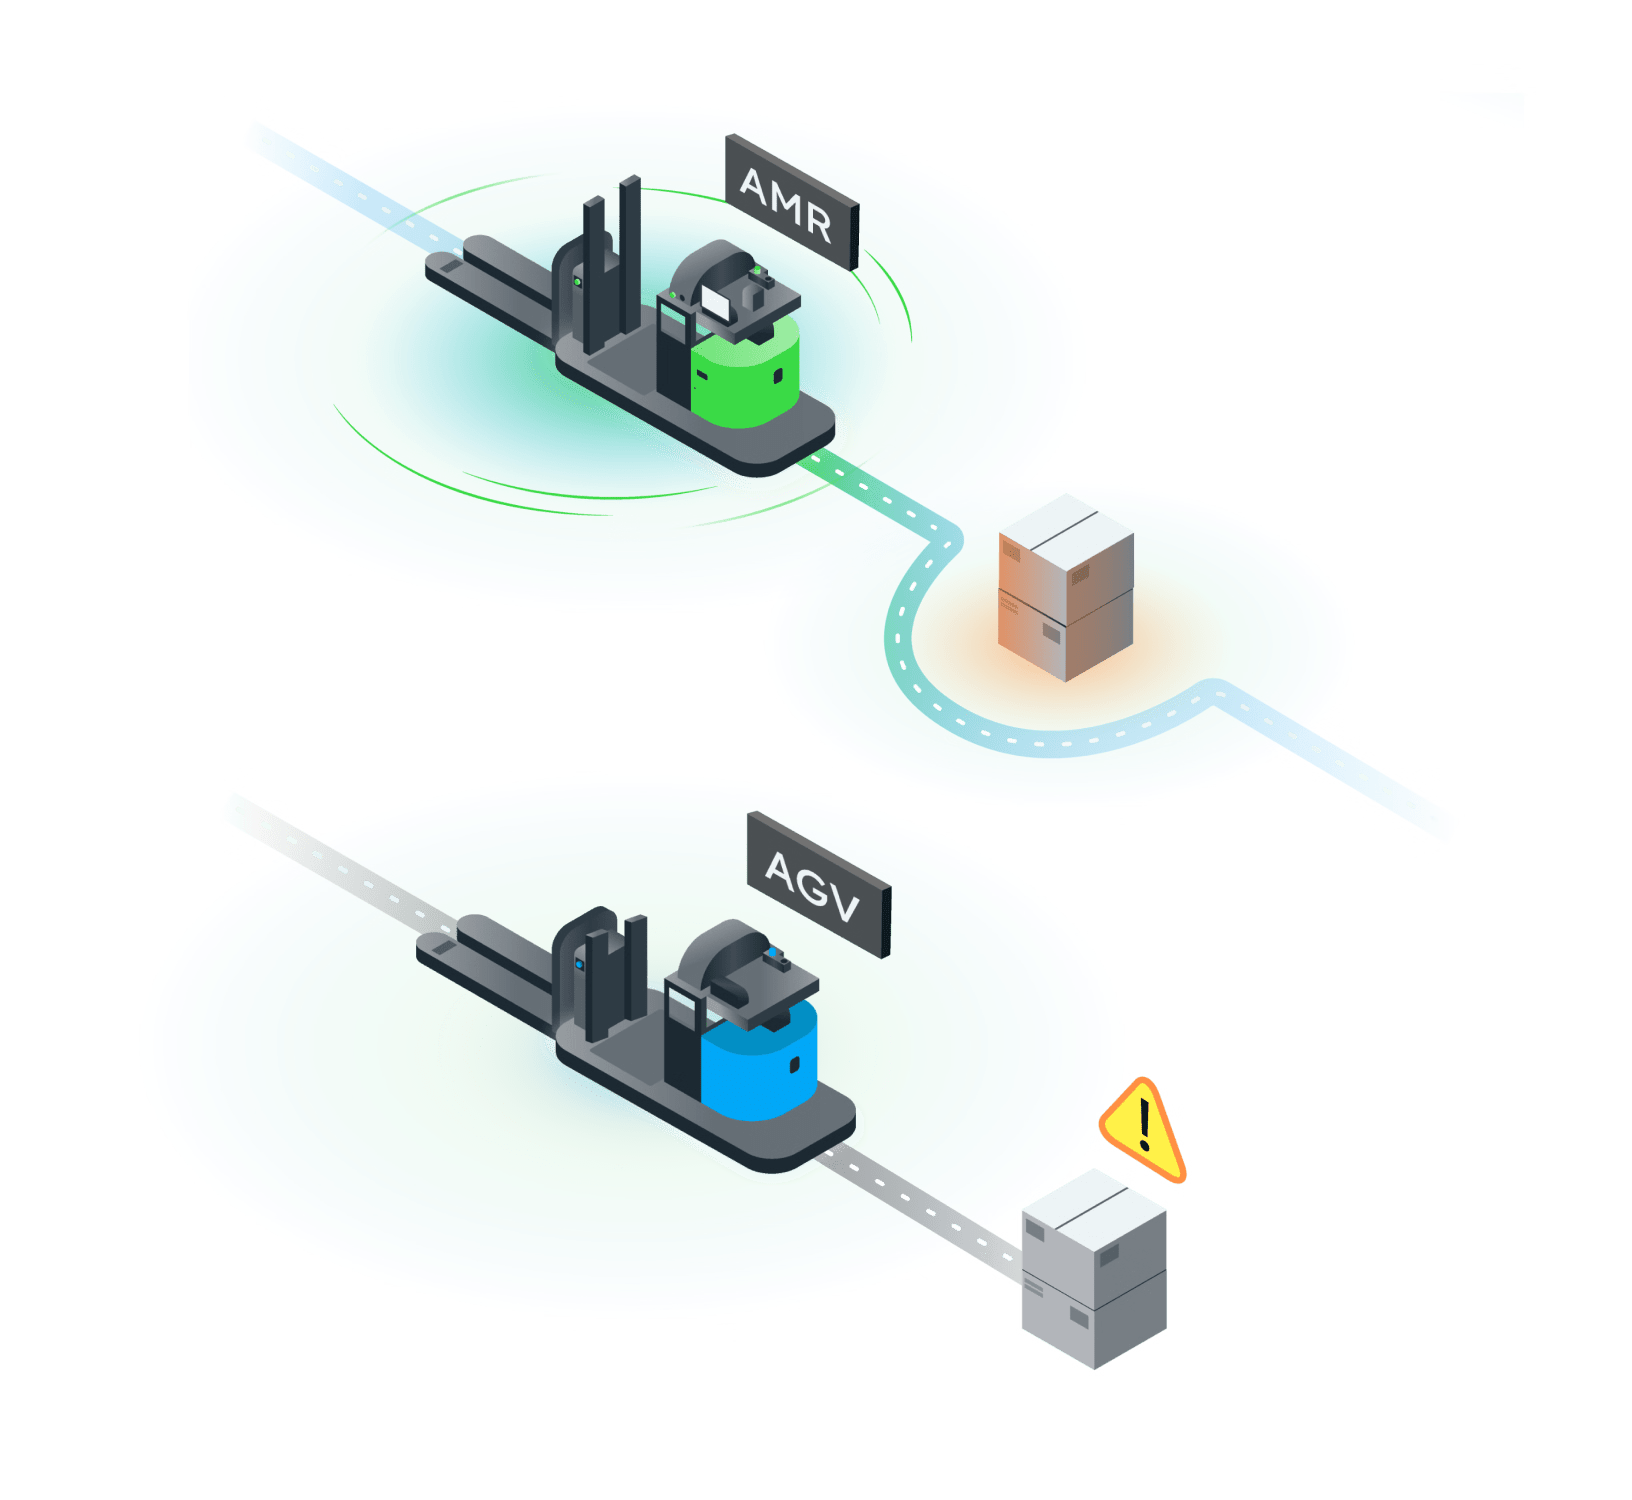
\includegraphics[width=5in]{images/Chap1/AMR-VS-AGV.png}\\
       \caption{AMR and AGV behaviors at presence of an obstacle \cite{R9}}
       \label{AMR-VS-AGV}
       \end{center}
\end{figure}

In addition, they grant a fast integration into new environments due to smart perception 
and recognition technologies. AMRs use this data as input to smart algorithms that 
enable it to plan its missions, navigate to its destination, avoid collisions, and 
execute missions all while collaborating with humans in the working space. The 
Autonomous vehicles do not require an automation expert or a roboticist’s presence to 
be configured or to deal with complex situations. It is able to solve such situations 
individually due to the scalable software that it has on board.

On the one hand, this evolution enables AMRs to navigate more dynamically and adaptively 
within intralogistics environments, improving overall efficiency and responsiveness. 
On the other hand, the level of flexibility that AMRs brings important safety and 
efficiency considerations \cite{R7}.

One of the main challenges is developing the navigation mechanisms. In a logistics 
environment, it is crucial to comply with the nature of the workspace. The AMR should 
recognize the location of materials to be handled and be able to navigate to and from 
those locations to next missions. Building a flexible and efficient solution requires a 
deep understanding of the situations and special cases that the vehicle may encounter 
and a study about how to create scalable solutions for such events.  

Before diving into the methodologies and technologies used to address this thesis’ 
topic, it is relevant to examine the related works. This research will serve later in 
the thesis as a guiding outline. Literature helps to investigate the level of progress that 
other researchers reached in similar topics, prevents re-invention of existing concepts, 
and pushes to ethically exploit the developed technologies. For this thesis, it is 
important to deeply examine the research papers and scientific resources to build a 
solid foundation of knowledge, identify the gaps in some studies, and propose novel 
solutions.  

In this context, this state-of-the-art report, delves 
into pathplanning and near-field path planning for mobile robots 
in general and for intralogistics AMRs specifically. Then, it examines possible 
solutions for path creation and generation. Afterwards, 
it studies the decision-making science approaches that can be used to evaluate and 
optimize path suggestions. Finally, this chapter 
outlines the methodology to be followed throughout this scientific work(Figure \ref{mindmap}).

\begin{figure}[H]
    \begin{center}
       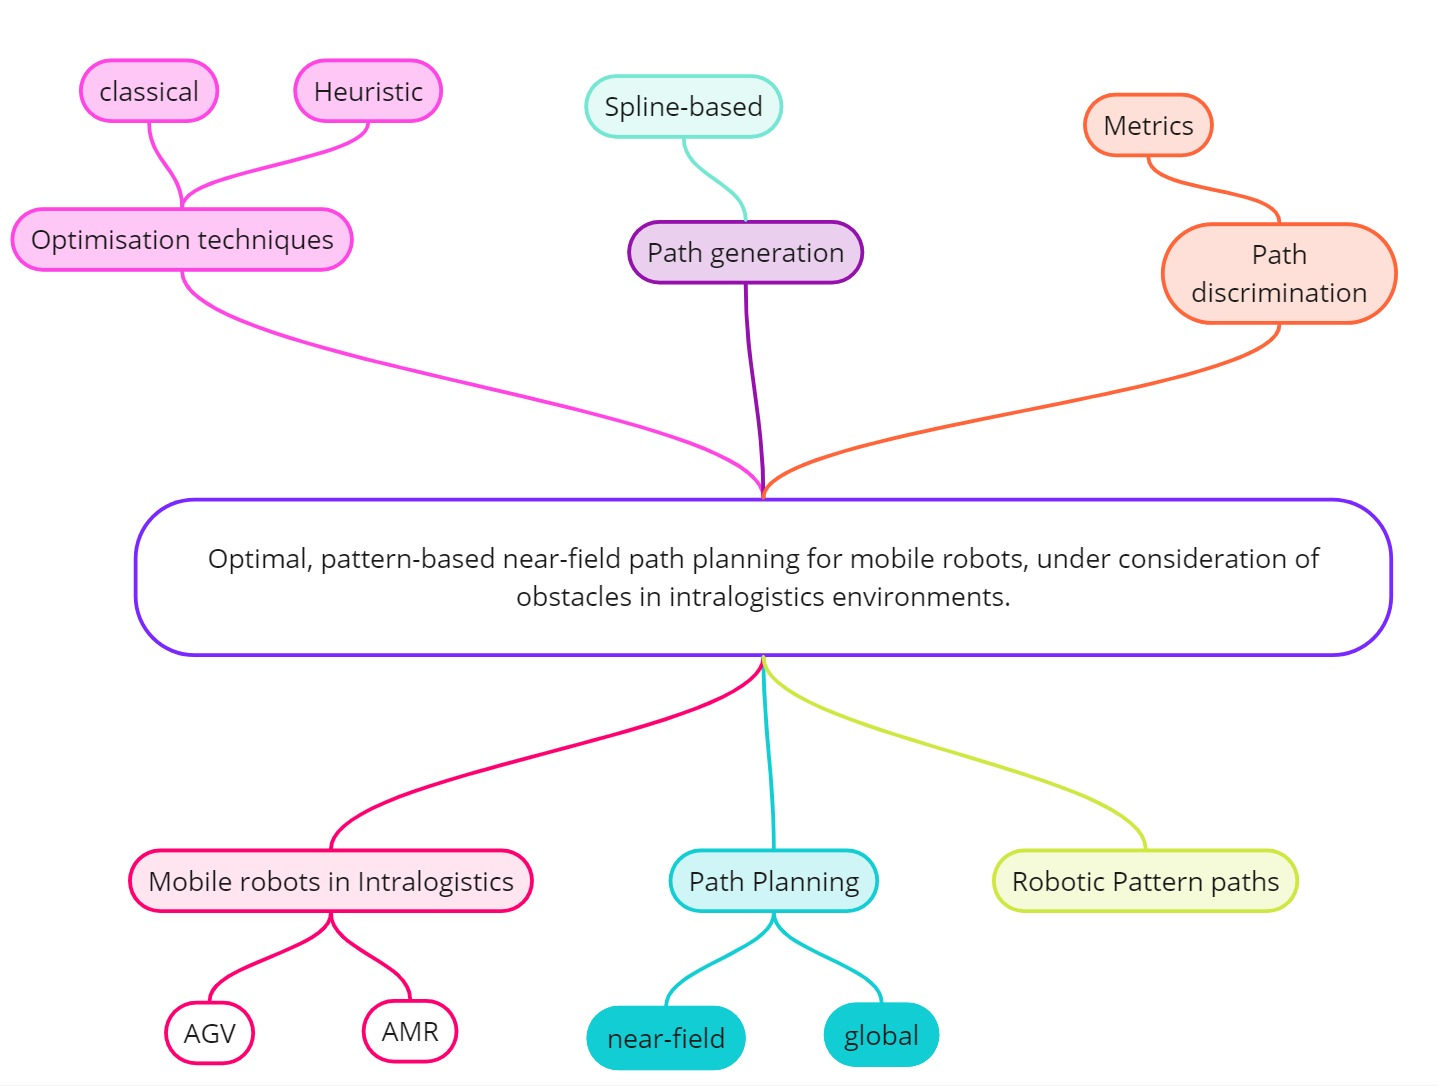
\includegraphics[width=6in]{images/Chap1/Fig1.jpg}\\
       \caption{Mind map of the key topics}
       \label{mindmap}
       \end{center}
\end{figure}

\newpage
\section{Path Planning}
